\documentclass[11pt, a4paper]{article}

\usepackage[T2A]{fontenc}		%cyrillic output
\usepackage[utf8]{inputenc}		%cyrillic output
\usepackage[english, russian]{babel}	%word wrap
\usepackage{amssymb, amsfonts, amsmath}	%math symbols
\usepackage{mathtext}			%text in formulas
\usepackage{geometry}			%paper format attributes
\usepackage{fancyhdr}			%header
\usepackage{graphicx}			%input pictures
\usepackage{tikz}				%draw pictures
\usetikzlibrary{patterns}		%draw pictures: fill
\usepackage{enumitem}			%enumarate parameters

\geometry{left=1cm, right=1cm, top=2cm, bottom=1cm, headheight=15pt}
\setlist[enumerate]{leftmargin=*}	%remove enumarate indenttion
\sloppy							%correct overfull

\newcommand{\head}[4]
{
	\pagestyle{fancy}
	\fancyhf{}
	\chead{#3, #4}

	\begin{center}
	\begin{large}
	#1 \\
	\textit{#2}\\
	\end{large}
	\end{center}

}

\begin{document}

\head{Открытая студенческая олимпиада по математике \\ Казахстанского филиала МГУ}{21 декабря 2012}{Казахстанский филиал МГУ имени М. В. Ломоносова}{г. Астана}

\begin{enumerate}

\item (Абдикалыков А.К.) Пусть $x$ --- вектор-столбец, все элементы которого равны 1, тогда произвольная целочисленная матрица $Q$ порядка $n$ будет <<весёлой>> тогда, и только тогда, когда вектор-столбец $Qx$ будет содержать только чётные числа. Возьмём теперь любую целочисленную матрицу $A$ и любую <<весёлую>> матрицу $B$, тогда все компоненты вектор-столбца $ABx=A(Bx)$ будут чётными, следовательно, матрица $AB$ --- <<весёлая>>.

\item $t$ является корнем $x^2 = 0$ тогда, и только тогда, когда $(t+1)$ является корнем $x^2 = 1$.

\item Обозначим через $F$ фокус параболы, через $H$ и $G$ --- проекции точек $A$ и $B$ на директрису параболы.

\begin{center}
%\input{solution/pictures/2012-2013-3}
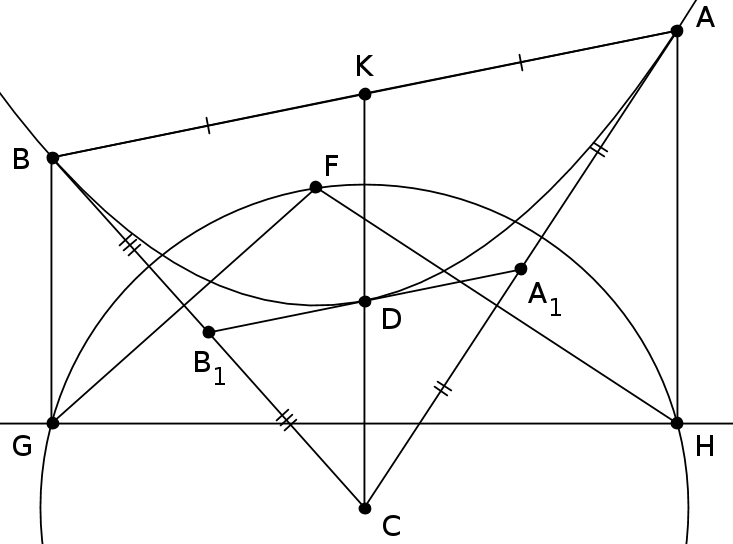
\includegraphics{pictures/2012-2013-3}
\end{center}

Свойство 1. $C$ --- центр описанной окружности треугольника $FGH$. Согласно оптическому свойству параболы: $AC$ --- биссектриса $\angle FAH$. А согласно определению $AF = AH$. Значит $AC$ --- серединный перпендикуляр к $FH$. Аналогично $BC$ --- серединный перпендикуляр к $FG$. 

Свойство 2. прямая $KC$ параллельна оси симметрии параболы и равноудалена от $AH$ и $BG$. Из свойства 1, $KC$ --- серединный перпендикуляр к $GH$. А точка $K$ равноудалена от прямых $AH$ и $BG$, поэтому $KC$ параллельна оси симметрии.

Обозначим $D$ --- точку пересечения $KC$ и параболы, $A_1$ и $B_1$ --- пересечение касательной к параболе в точке $D$ c прямыми $CA$ и $CB$. 

Свойство 3. $A_1B_1$ --- средняя линия треугольника $ABC$. Согласно свойству 2, $A_1$ равноудалена от прямых $KC$ и $AH$, а $B_1$ равноудалена от $KC$ и $BG$. Значит, $AA_1 = A_1C$ и $BB_1 = B_1C$. 

\item (Абдикалыков А.К.) Ответ: 4, 5, 6, 7. Перепишем это равенство в виде $\displaystyle\sum\limits_{k=2}^n{\left[\sqrt[k]{n}~\right]}=n$. В левой части полученного соотношение находится сумма $n-1$ натурального числа, расположенного в порядке невозрастания, следовательно, $\left[\sqrt{n}~\right]=2$, $\left[\sqrt[3]{n}~\right]=1$. Выводим $n\in\left\{4, 5, 6, 7\right\}$; все эти значения удовлетворяют исходному равенству.


\item Ответ: 981. Подходящие числа записываются в троичной системе счисления только цифрами 0 и 1. Таким образом, запись искомого числа в троичной системе счисления совпадает с двоичной записью числа 100: $$100 = 64 + 32 + 4 = 1100100_2.$$
Ответ на задачу: $$3^6 + 3^5 + 3^2 = 729 + 243 + 9 = 981.$$

\item Умножив обе части данного равенства на $A^n$ слева, получим $a_0=0$ и исключим единичную матрицу из равенства. Умножим теперь то же равенство на $A^{n-1}$, получим $a_1=0$ и исключим уже $A$ в первой степени. Продолжая этот процесс, получим требуемое. Доказательство утверждения в обратную сторону тривиально.

\item Ответ: $\frac{4}{3} (\pi^2 - 9)$. Достаточно воспользоваться тождеством:
$$\frac{1}{1^3 + 2^3 + \hdots + k^3} = 4 \left(\frac{1}{k} - \frac{1}{k+1}\right)^2.$$

\item Никакие две из указанных 12 клеток не могут быть заняты или быть побиты одним конем.

\begin{center}
\begin{tikzpicture}[x=8,y=8]
\draw[step=1] (0,0) grid (8, 8);
\draw[fill] (0,0) rectangle (1, 1);
\draw[fill] (0,1) rectangle (1, 2);
\draw[fill] (1,1) rectangle (2, 2);

\draw[fill] (6,1) rectangle (7, 2);
\draw[fill] (6,0) rectangle (7, 1);
\draw[fill] (7,0) rectangle (8, 1);

\draw[fill] (6,6) rectangle (7, 7);
\draw[fill] (7,6) rectangle (8, 7);
\draw[fill] (7,7) rectangle (8, 8);

\draw[fill] (0,7) rectangle (1, 8);
\draw[fill] (1,7) rectangle (2, 8);
\draw[fill] (1,6) rectangle (2, 7);
\end{tikzpicture}
\end{center}

\item Воспользуемся неравенством:
$$\int\limits_{0}^{1} \left(f(x) - ax - b\right)^2\,dx \geqslant 0,$$
которое верно для любых $a, b \in \mathbb{R}$. $a$ и $b$ выбираются соответствующим образом.

\end{enumerate}



\end{document} 
